\documentclass[12pt]{article}  % standard LaTeX, 12 point type
\usepackage{amsfonts,latexsym}
\usepackage{amsthm}
\usepackage{amssymb}
\usepackage[utf8]{inputenc} % Кодировка
\usepackage[english,russian]{babel} % Многоязычность

\newtheorem{theorem}{Theorem}[section]
\newtheorem{proposition}[theorem]{Proposition}
\newtheorem{lemma}[theorem]{Lemma}
\newtheorem{corollary}[theorem]{Corollary}
\newtheorem{conjecture}[theorem]{Conjecture}

\theoremstyle{definition}
\newtheorem{definition}{Определение}[section]
\newtheorem{example}{Example}[section]

% unnumbered environments:

\theoremstyle{remark}
\newtheorem*{remark}{Remark}
\newtheorem*{notation}{Notation}
\newtheorem*{note}{Note}

\setlength{\parskip}{5pt plus 2pt minus 1pt}
\setlength{\parindent}{0pt}

\usepackage{color}
\usepackage{listings}
\usepackage{caption}
\usepackage{graphicx}

\graphicspath{{pics/}}


% \newcounter{nalg}[section] % defines algorithm counter for chapter-level
% \renewcommand{\thenalg}{\thechapter .\arabic{nalg}} %defines appearance of the algorithm counter
% \DeclareCaptionLabelFormat{algocaption}{Algorithm \thenalg} % defines a new caption label as Algorithm x.y

\lstnewenvironment{algorithm}[1][] %defines the algorithm listing environment
{   
    % \refstepcounter{nalg} %increments algorithm number
    % \captionsetup{labelformat=algocaption,labelsep=colon} %defines the caption setup for: it ises label format as the declared caption label above and makes label and caption text to be separated by a ':'
    \lstset{ %this is the stype
        frame=tB,
        numbers=left, 
        mathescape=true,
        numberstyle=\small,
        basicstyle=\small, 
        keywordstyle=\color{black}\bfseries,
        keywords={,function, procedure, return, datatype, function, in, if, else, for, foreach, while, begin, end, denote, do, and, then,} %add the keywords you want, or load a language as Rubens explains in his comment above.
        numbers=left,
        xleftmargin=.04\textwidth,
        #1 % this is to add specific settings to an usage of this environment (for instnce, the caption and referable label)
    }
}
{}

\newcommand{\tab}[1][0.3cm]{\ensuremath{\hspace*{#1}}}





\title{Modification of modificated CYK}
\author{Anya Yaveyn}
\date{\today}

\begin{document}

Введем обозначения, немного отличающиеся от используемых в статье (Охотин, 2013).
Пусть $G=(\Sigma, N, R, S)$ --- грамматика и $w = a_0 \dots a_{n-1}$ --- строка, причем $n + 1 = 2^k$. $T$ --- треугольная матрица $n \times n$ с элементами $T[i,j] \subseteq N$. Цель алгоритма --- заполнить ячейки матрицы $T$ так, что будет выполняться
$$
T[i,j] = \{A\,|\,a_{n-1-j} \dots a_{i} \in L(A)\}, \tab \mbox{при } 0 \leqslant i, j \leqslant n-1 \leqslant i+j\,.
$$
Вторая матрица $P$ с элементами $P[i,j] \subseteq N \times N$ в результате должна быть заполнена значениями 
$$
P[i,j] = \{(B,C)\, |\, a_{n-1-j} \dots a_{i} \in L(B)L(C)\}, \tab 0 \leqslant i, j \leqslant n-1 \leqslant i+j\,.
$$

\begin{definition}
Назовем \textit{(квадратной) подматрицей} такой набор пар индексов $S=\{(i,j)\}$, что для каких-то $0 \leqslant a, b\leqslant n-1 \leqslant a+b$ и $0 < size \leqslant n-a,n-b$  любая пара $(i,j)$, удовлетворяющая условиям $a \leqslant i < a + size$ и $b \leqslant j < b + size$, принадлежит множеству $S$. Тогда $size$ --- \textit{размер}, а пара индексов $(a,b)$ --- \textit{вершина} этой подматрицы.
\end{definition}


\begin{figure}[!ht]
  \caption{Иллюстрация к определению.}
  \label{gr:submatrix}
  \centering
    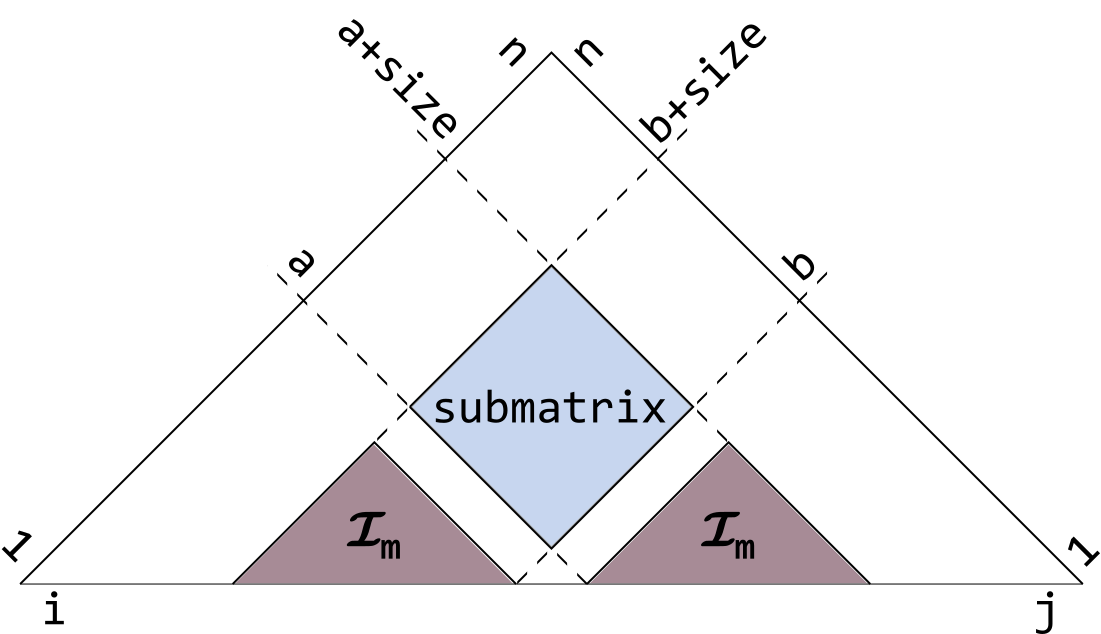
\includegraphics[width=0.9\linewidth]{submatrix.png}
\end{figure}


\begin{definition}
Пусть $S$ --- подматрица. Будем обозначать через $T[S]$ и $P[S]$ подматрицы матриц $T$ и $P$, соответствующие множеству индексов $S$.
\end{definition}

Для написания алгоритма нам в первую очередь необходимо задать структуру для представления подматриц и определить для этой структуры следующие функции.

\begin{algorithm}[caption={Submatrix helpers.}, label={helpers}]
function size(submatrix)
function vertex(submatrix)

function leftSubmatrix(submatrix)
function topSubmatrix(submatrix)
function rightSubmatrix(submatrix)
function bottomSubmatrix(submatrix)

function rightNeighbor(submatrix)
function leftNeighbor(submatrix)
function rightGrounded(submatrix)
function leftGrounded(submatrix)     
\end{algorithm}

Здесь, функции size и vertex возвращают соответственно размер и вершину подматрицы. Следующие четыре функции leftSubmatrix ---\linebreak bottomSubmatrix возвращают одну из подматриц, делящих исходную подматрицу на четыре части, как показано на рисунке \ref{gr:inner}.


\begin{figure}[!ht]
  \caption{Иллюстрация к листингу.}
  \label{gr:inner}
  \centering
    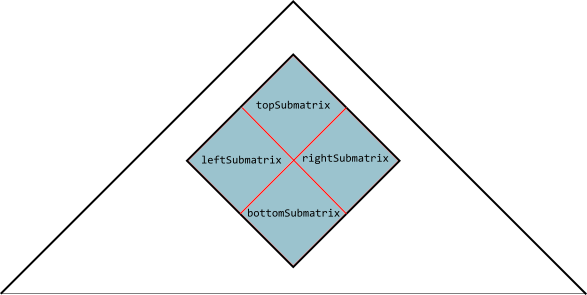
\includegraphics[width=0.9\linewidth]{inner.png}
\end{figure}

\pagebreak

В свою очередь функции rightNeighbor --- leftGrounded возвращают подматрицы, сдвинутые относительно исходной так, как показано на рисунке \ref{gr:outer}.

\begin{figure}[!ht]
  \caption{Иллюстрация к листингу.}
  \label{gr:outer}
  \centering
    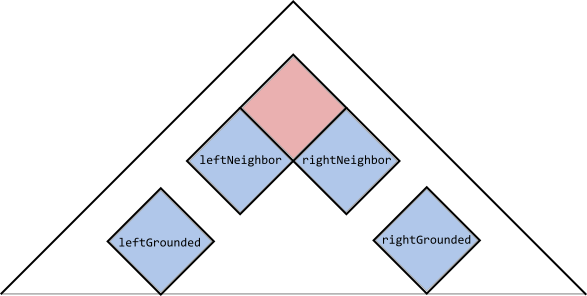
\includegraphics[width=0.9\linewidth]{outer.png}
\end{figure}

Теперь можно приступить к описанию самого алгоритма. Он состоит из трех процедур.

Главная процедура main сначала обрабатывает нижний слой матрицы $T$ (клетки $(i,j)$, для которых $i+j=n-1$), записывая в него корректные значения. Потом разбивает матрицу $T$ на слои, как показано на картинке \ref{gr:layers} (каждый слой по сути состоит из набора подматриц, у каждой из которых отброшена нижняя четверть --- bottomSubmatrix). Полученные слои обрабатываются последовательно снизу вверх, с помощью процедуры completeVLayer, заполняя тем самым всю матрицу $T$. 

\begin{figure}[!ht]
  \caption{Первичное разбиение на слои.}
  \label{gr:layers}
  \centering
    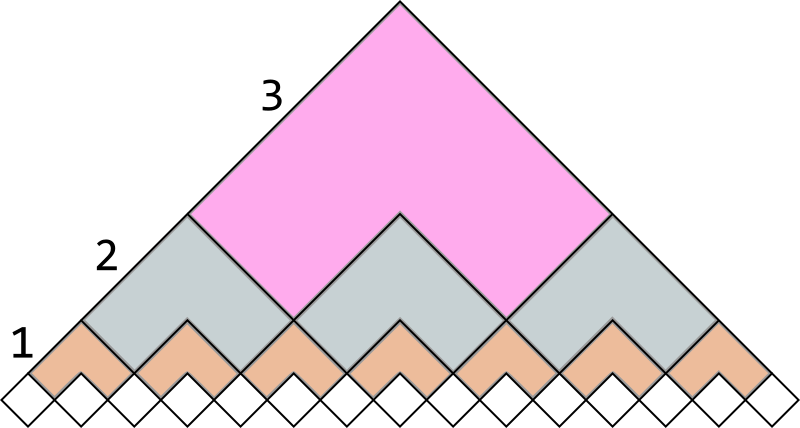
\includegraphics[width=0.9\linewidth]{layers.png}
\end{figure}

Процедура completeVLayer, в свою очередь, принимает на вход набор подматриц $M$. Для каждого элемента $m$ этого набора процедура достраивает матрицу $T$ для трех верхних четвертей (leftSubmatrix$(m)$, \linebreak rightSubmatrix$(m)$ и topSubmatrix$(m)$). Для корректной работы этой функции необходимо, чтобы для любой $m \in M$ ячейки $T[i,j]$ были построены  для $(i,j) \in\ $bottomSubmatrix$(m)$, а также для таких $(i,j)$, что $i < a, j < b+s$ или $i < a+s, j < b$, где $(a,b)$ --- вершина, а $s$ --- размер подматрицы $m$. 

Третья процедура --- completeLayer --- тоже принимает на вход набор подматриц $M$, но для каждого элемента $m$ этого набора достраивает матрицу $T$ для всей подматрицы $m$. Для корректной работы этой функции требуется, чтобы для любой $m \in M$ ячейки $T[i,j]$ были построены для таких $(i,j)$, что $i < a, j < b+s$ или $i < a+s, j < b$, где $(a,b)$ --- вершина, а $s$ --- размер подматрицы $m$. 

\begin{algorithm}[caption={Algorithm.}, label={main}]
procedure main():
  for $\ell$ in $(0,\,\dots,\,n-1)$ do
    $T[\ell, n-1-\ell] = \{A\,|\,A \to a_{\ell} \in R\}$
  for i in 1 .. k-1 do
    denote layer = constructLayer(i)
    completeVLayer(layer)  

procedure completeLayer($M$):
  if $m \in M$ and size($m$) = 1 then
    denote cells = $\{$vertex$(m)\,|\, m \in M\}$
    foreach $(x, y) \in $ cells do
      T[x, y] = f(P[x, y])
  else
    denote bottomLayer = $\{$bottomSubmatrix$(m)\,|\,m \in M\}$
    completeLayer(bottomLayer)
    completeVLayer($M$)     

procedure completeVLayer($M$):
  denote leftSubLayer = $\{$leftSubmatrix$(m)\,|\,m \in M\}$
  denote rightSubLayer = $\{$rightSubmatrix$(m)\,|\,m \in M\}$
  denote topSubLayer = $\{$topSubmatrix$(m)\,|\,m \in M\}$

  foreach $m \in$ leftSubLayer do
    P[m] = P[m] $\cup$ (T[leftGrounded(m)] $\times$ T[rightNeighbor(m)])
  foreach $m \in$ rightSubLayer do
    P[m] = P[m] $\cup$ (T[leftNeighbor(m)] $\times$ T[rightGrounded(m)])

  completeLayer(leftSubLayer $\cup$ rightSubLayer)

  foreach $m \in$ topSubLayer do
    P[m] = P[m] $\cup$ (T[leftGrounded(m)] $\times$ T[rightNeighbor(m)])
  foreach $m \in$ topSubLayer do
    P[m] = P[m] $\cup$ (T[leftNeighbor(m)] $\times$ T[rightGrounded(m)])

  completeLayer(topSubLayer)  
\end{algorithm}

Процедура main реализуется через completeVLayer очевидным образом. completeLayer по сути аналогична процедуре complete из статьи, за исключением того, что она выполняется сразу для нескольких матриц. Таким же образом отдельно разбирается случай, когда переданные матрицы имеют размер один. Иначе матрицы разбиваются на четыре части и сначала следует рекурсивный вызов от bottomSubmatrix (для всех переданных матриц), а потор вызов процедуры completeVLayer, которая обрабатывает верхние части матриц. 

completeVLayer для каждой из переданных матриц сначала выполняет два перемножения (соответствует 14 и 16 строкам в алгоритме из статьи), потом вызывает completeLayer от rightSubmatrix и leftSubmatrix (15 и 17 строки оригинального алгоритма), далее выполняет оставшиеся два умножения (строки 18 и 19) и, наконец, вызывает completeLayer от оставшейся части topSubmatrix (строка 20).






\end{document}